\section{Analysis}
\label{sec:analysis}

\subsection{Reward and Accuracy Progression Across Generations}

To better understand the dynamics of skill evolution, we analyze both the per-task running mean reward and running accuracy across generations (\Cref{fig:combined}). The reward curve reflects the average verifier score over rollout populations, while the accuracy curve indicates whether at least one rollout successfully solves a task. Although rewards are binary in our setting, the two metrics capture different aspects of performance. Reward reflects the consistency of successful rollouts within a task, whereas accuracy measures only whether a task is solved at least once. As a result, the two trends are correlated but not identical, providing complementary views of both capability and reliability.

\begin{figure}[ht]
    \centering
    % \begin{subfigure}{0.49\linewidth}
    %     \centering
    %     \includegraphics[width=\linewidth]{figures/mean_reward_by_step.pdf}
    %     \caption{Mean rewards across generations}
    %     \label{fig:mean_rewards_per_gen}
    % \end{subfigure}
    % \hfill
    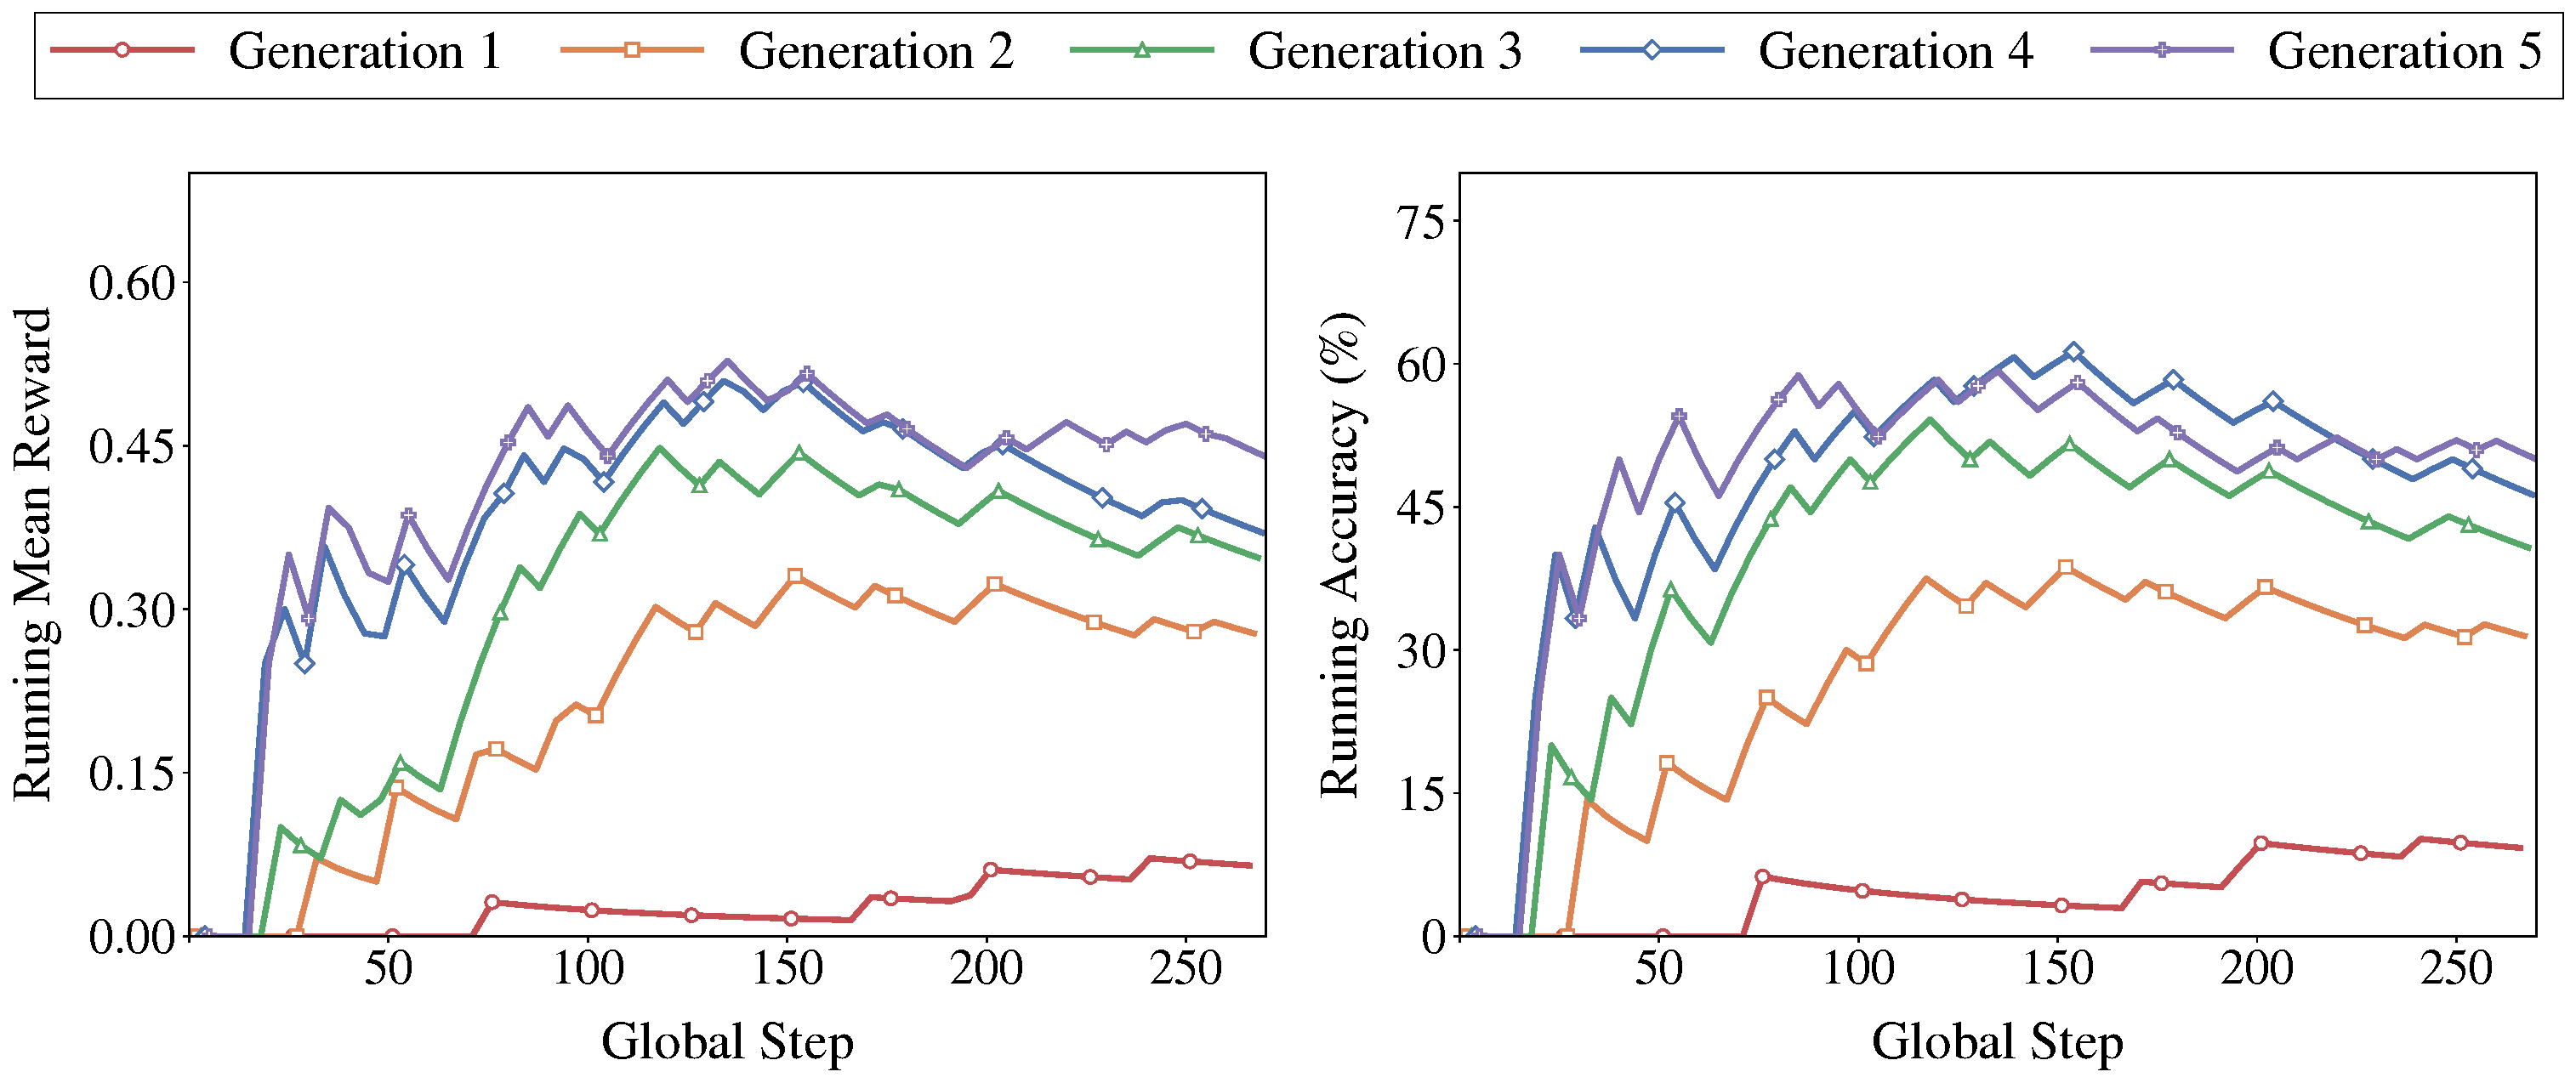
\includegraphics[width=\linewidth]{figures/combined_figure.pdf}
    % \caption{Accuracy across generations}
    % \label{fig:accuracy_per_gen}
    \caption{Accuracy and reward curves across 5 generations. }
    \label{fig:combined}
    \vspace{-1em}
\end{figure}

The two figures reveal a clear and largely monotonic ordering after the initial warm-up: Generation~5 outperforms Generation~4, which outperforms Generation~3, and so on, but the magnitude of improvement is not uniform across generations. The largest gains occur between Generations~1 and~3, where both reward and accuracy increase sharply as useful skills begin to transfer across tasks. By the end, Generation~5 reaches a running mean reward of $0.44$ and accuracy of $50.0\%$, compared to $0.06$ reward and $9.3\%$ accuracy for Generation~1, while Generation~4 achieves $0.37$ and $46.3\%$. This pattern suggests that most of the broad performance gains are realized by the first three generations, while Generations~4 and~5 increasingly plateau and primarily refine an already strong skill set rather than opening up a comparably new level of capability.

Comparing reward and accuracy further clarifies this behavior. The larger improvement in reward than accuracy from Generation~4 to~5 indicates that later generations improve consistency rather than merely solving additional tasks. Once a task becomes solvable, they increase the likelihood that sampled rollouts succeed, enhancing reliability within each task. The largest jump still occurs between the early generations, especially from Generation~1 to Generations~2 and~3, indicating that the highest-value skill repairs are discovered early. Later generations improve more modestly, but the accuracy panel shows that those improvements remain meaningful rather than cosmetic. This suggests that a small number of editing rounds captures the majority of improvements, with additional iterations yielding incremental but meaningful gains in robustness and coverage.

\subsection{Qualitative Analysis}
% \subsubsection{Trained v/s Inference Skill Editor}
% The performance gap between Skill-R1 (GRPO Editor) and Skill-R1 (Inference Editor) in \Cref{tab:main_results} reflects a deeper difference in what each editor learns to treat as signal. At a high level, the comparison is between two editing behaviors: one that treats rollout evidence as a cue for selective repair, and one that absorbs incidental context and drifts toward overfitting. The \texttt{pdb} skill is a useful lens on this distinction because it begins as a broad reference document, covering BioPython workflows, structure traversal, coordinate extraction, distance computation, ligand handling, and manual parsing. It is written as a general-purpose manual rather than a task-specific policy.

% When both editors are exposed to rollout evidence containing a genuine PDB failure together with unrelated nearby context, the trained editor responds conservatively. It preserves the basic structure of the skill, retains executable BioPython examples, and inserts targeted safeguards around actual failure points, such as missing dependencies, missing files, and empty models or chains. Even when the rollout contains evidence about misuse, that information remains peripheral. The resulting artifact is still recognizably a PDB skill: narrower and more robust than the original, but still broadly applicable to novel structure-analysis queries.

% The inference-only editor behaves very differently. Instead of repairing the skill while preserving its executable core, it rewrites the document around the incidental details of the sampled rollout. In the extreme case, it treats an internal benchmark identifier as though it were a malformed PDB accession and devotes substantial space to rejecting an unrelated audio query. The Quick Start and code examples disappear entirely, replaced by benchmark-shaped warnings and verbose instructions anchored to a small number of observed failures. The result is not a repaired skill but an overfit response policy whose content is dominated by accidental co-occurrence.

% This contrast clarifies why reward-trained editing outperforms inference-only editing. Without a cross-task reward signal, inference-time revision has no reliable mechanism for separating transferable structure from coincidental context. GRPO changes that inductive bias. Because the editor is optimized against bi-level advantages aggregated across rollouts, it is encouraged to preserve what continues to work across tasks and to modify only those parts of the skill that systematically limit reward. The learned behavior is therefore not simply ``more cautious'' editing; it is editing that is selective about what deserves to be remembered. Full skill listings for both the GRPO-edited and inference-edited \texttt{pdb} skill (alongside the original) are provided in \Cref{app:pdb_skill_comparison}.

% \subsubsection{Editing Trajectory Across Generations}
% Tracing the same skill across generations reveals a second qualitative pattern. Skill evolution is not a story of monotonic accumulation, where each round simply appends more advice to an already long document. Instead, the editor first compresses broad, tutorial-like skills into shorter executable routines, then sharpens them around recurrent failure modes, and finally stabilizes them with stronger task-boundary guardrails. The overall effect is a prune-then-specialize dynamic in which general reference material is gradually displaced by compact instructions that are easier to deploy under the distribution of tasks encountered during training.

% The \texttt{pdb} skill provides a concrete illustration of this progression. In its original form, the skill reads like a general-purpose reference manual, containing multiple BioPython workflows, file-format documentation, and manual parsing utilities. By the first generation, that broad reference has already been condensed into a single distance-computation workflow accompanied by a short list of concrete best practices. In the second generation, the skill narrows further: background exposition is stripped away, and the document is reorganized around local-file handling, explicit error checks, and tightly specified output behavior. By the third generation, the skill no longer resembles a general primer. It functions instead as a compact policy, retaining only a small executable core while adding stronger misuse guardrails, including an explicit rejection of an unrelated audio-file query. This complements the trained-vs.-inference comparison above. GRPO training curbs the most pathological forms of overfitting seen in inference-only editing, but it does not eliminate task conditioning altogether. Over longer horizons, the dominant trend is a shift away from general-purpose documentation and toward compact, deployment-oriented artifacts that increasingly reflect the recurrent structure of the training distribution. 

\subsubsection{Trained v/s Inference Skill Editor}

The performance gap between Skill-R1 (GRPO) and Skill-R1 (Inference) in \Cref{tab:main_results,tab:webwalker_results} reflects a fundamental difference in how each editor interprets rollout evidence. The trained editor treats rollouts as signals for targeted repair, while the inference-only editor tends to overfit to incidental context.

Using the \texttt{pdb} skill as a case study, the trained editor preserves the core executable structure and introduces focused safeguards around genuine failure modes (e.g., missing files or dependencies). In contrast, the inference-only editor rewrites the skill around spurious details from sampled rollouts, often discarding essential components such as executable code. This leads to brittle, task-specific artifacts that fail to generalize.

This qualitative difference is reflected in performance, while inference-only Skill-R1 provides modest gains over Vanilla GRPO on GAIA (30.9\% vs. 29.7\%), it underperforms on WebWalker (19.0\% vs. 22.0\%), the GRPO-trained editor consistently improves performance across benchmarks (41.8\% on GAIA and 26.0\% on WebWalker), demonstrating that reward driven editing better captures transferable structure.

Overall, training enables selective retention of useful behaviors while suppressing noise, leading to more robust and generalizable skill updates. Full skill listings for both the GRPO-edited and inference-edited \texttt{pdb} skill (alongside the original) are provided in \Cref{app:pdb_skill_comparison}.

\subsubsection{Editing Trajectory Across Generations}

Skill evolution follows a structured progression rather than simple accumulation. Early generations yield the largest gains by correcting high-impact errors, as also reflected in the sharp improvements from Generation 1 to 3 in \Cref{fig:combined}. Later generations provide smaller but consistent improvements by refining reliability and stabilizing behavior.

Qualitatively, this corresponds to a prune then specialize dynamic. Initial skills, which resemble broad reference documents, are quickly compressed into shorter executable routines. Subsequent generations focus on recurring failure modes and introduce tighter constraints and guardrails, resulting in compact, deployment oriented policies.

This pattern aligns with the quantitative trends: most performance gains are realized early, while later iterations primarily improve consistency rather than expanding capability. Together, these observations suggest that multi-generation evolution is effective not only for discovering better skills, but also for making them more reliable under repeated execution.